\documentclass{echw}

\title{Tutorial A10.4\\Complex Numbers}
\author{Eytan Chong}
\date{2024-07-08}

\begin{document}
    \problem{}
        A complex number $z$ is represented in an Argand diagram by the point P. Sketch, on separate Argand diagrams, the locus of $P$. Describe geometrically the locus of $P$ and determine its Cartesian equation.

        \begin{enumerate}
            \item $\abs{2z - 6 - 8i} = 10$
            \item $\abs{z + 2} = \abs{z - i}$
            \item $\arg{z + 2 - i} = -\dfrac\pi4$
        \end{enumerate}

    \solution
        \part
            Note that $\abs{2z - 6 - 8i} = 10 \implies \abs{z - (3 + 4i)} = 5$.

            \begin{center}
                \begin{tikzpicture}[trim axis left, trim axis right]
                    \begin{axis}[
                        domain = 0:10,
                        samples = 101,
                        axis y line=middle,
                        axis x line=middle,
                        xtick = \empty,
                        ytick = \empty,
                        xmax=11.5,
                        xmin=-5.5,
                        ymin=-4,
                        ymax=11,
                        xlabel = {$\Re$},
                        ylabel = {$\Im$},
                        legend cell align={left},
                        legend pos=outer north east,
                        after end axis/.code={
                            \path (axis cs:0,0) 
                                node [anchor=north east] {$O$};
                            }
                        ]
            
                        \coordinate (O) at (0, 0);
                        \coordinate[label=right:$3 + 4i$] (C) at (3, 4);

                        \fill (C) circle[radius=2.5pt];

                        \draw[<->] (O) -- (C);

                        \node[anchor=west] at (1.7, 2) {$5$};

                        \draw[plotRed] (C) circle[radius=5];
                        
                        \addlegendimage{no markers, plotRed}
                        \addlegendentry{locus of $P$};
                    \end{axis}
                \end{tikzpicture}
            \end{center}

            \boxt{\begin{center}The locus of $P$ is a circle with centre $(3, 4)$ and radius $5$.\\Its Cartesian equation is $(x-3)^2 + (y-4)^2 = 5^2$.\end{center}}

        \part
            Note that $\abs{z + 2} = \abs{z - i} \implies \abs{z - (-2)} = \abs{z - i}$.

            \begin{center}
                \begin{tikzpicture}[trim axis left, trim axis right]
                    \begin{axis}[
                        domain = -10:10,
                        samples = 101,
                        axis y line=middle,
                        axis x line=middle,
                        xtick = {-2},
                        ytick = {1},
                        yticklabels = {$i$},
                        xmax=2,
                        xmin=-3,
                        ymin=-2,
                        ymax=2,
                        xlabel = {$\Re$},
                        ylabel = {$\Im$},
                        legend cell align={left},
                        legend pos=outer north east,
                        after end axis/.code={
                            \path (axis cs:0,0) 
                                node [anchor=north west] {$O$};
                            }
                        ]
            
                        \coordinate (Z1) at (-2, 0);
                        \coordinate (Z2) at (0, 1);
                        \coordinate (O) at (0, 0);

                        \draw[dotted] (Z1) -- (Z2);

                        \addplot[plotRed] {-2*x - 1.5};
                
                        \fill (Z1) circle[radius=2.5pt];
                        \fill (Z2) circle[radius=2.5pt];

                        \addlegendentry{locus of $P$};

                        \coordinate (Z3) at (0, -1.5);
                        \coordinate (Z4) at (-1, 0.5);
                        \draw pic [draw, angle radius=3mm, ""] {right angle =  Z3--Z4--Z2};
                    \end{axis}
                \end{tikzpicture}
            \end{center}

            \boxt{\begin{center}The locus of $P$ is the perpendicular bisector of the line segment joining \\$(-2, 0)$ and $(0, 1)$. Its Cartesian equation is $y = -2x - 1.5$.\end{center}}

        \part
            Note that $\arg{z + 2 - i} = -\dfrac\pi4 \implies \arg{z - (-2 + i)} = -\dfrac\pi4$.

            \begin{center}
                \begin{tikzpicture}[trim axis left, trim axis right]
                    \begin{axis}[
                        domain = -2:3,
                        samples = 101,
                        axis y line=middle,
                        axis x line=middle,
                        xtick = {-2},
                        ytick = {1},
                        yticklabels = {$i$},
                        xmax=2,
                        xmin=-3,
                        ymin=-2,
                        ymax=2,
                        xlabel = {$\Re$},
                        ylabel = {$\Im$},
                        legend cell align={left},
                        legend pos=outer north east,
                        after end axis/.code={
                            \path (axis cs:0,0) 
                                node [anchor=north west] {$O$};
                            }
                        ]
            
                        \coordinate[label=above:$-2+i$] (Z1) at (-2, 1);
                        \coordinate (Z2) at (0, 1);
                        \coordinate (O) at (0, 0);

                        \draw[dotted] (Z1) -- (Z2);

                        \addplot[plotRed] {-x - 1};
                
                        \draw (Z1) circle[radius=2.5pt];

                        \addlegendentry{locus of $P$};

                        \coordinate (Z3) at (0, -1);
                        \draw pic [draw, angle radius=12mm, "$-\frac\pi4$"] {angle =  Z3--Z1--Z2};
                    \end{axis}
                \end{tikzpicture}
            \end{center}
            
            \boxt{\begin{center}The locus of $P$ is the half-line starting from $(-2, 1)$ and inclined at an angle $-\dfrac\pi4$ to the positive real axis. Its Cartesian equation is $y = -x - 1$.\end{center}}


    \problem{}
        Sketch the following loci on separate Argand diagrams.

        \begin{enumerate}
            \item $\Re{z^2} = 1$
            \item $\abs{6 - iz} = 2$,
            \item $\arg{\dfrac{iz}{1 - \sqrt3 i}} = \pi$
        \end{enumerate}

    \solution
        \part
            Let $z = r(\cos \t + i\sin \t)$. Then $\Re{z^2} = 1 \implies r^2 \cos 2\t = 1 \implies r^2 = \sec 2\t$.

            \begin{center}
                \begin{tikzpicture}[trim axis left, trim axis right]
                    \begin{axis}[
                        domain = 0:2*pi,
                        samples = 100,
                        axis y line=middle,
                        axis x line=middle,
                        xtick = {-1, 1},
                        ytick = \empty,
                        xmin=-2,
                        xmax=2,
                        ymin=-2,
                        ymax=2,
                        xlabel = {$\Re$},
                        ylabel = {$\Im$},
                        legend cell align={left},
                        legend pos=outer north east,
                        after end axis/.code={
                            \path (axis cs:0,0) 
                                node [anchor=north east] {$O$};
                            }
                        ]
                        \addplot[color=plotRed,data cs=polarrad] {1/sqrt(cos(2 * \x r))};
            
                        \addlegendentry{required locus};
                    \end{axis}
                \end{tikzpicture}
            \end{center}

        \part
            Note $\abs{6 - iz} = 2 \implies \abs{-i (z + 6i)} = 2 \implies \abs{z + 6i} = 2 \implies \abs{z - (6i)} = 2$.

            \begin{center}
                \begin{tikzpicture}[trim axis left, trim axis right]
                    \begin{axis}[
                        domain = 0:10,
                        samples = 101,
                        axis y line=middle,
                        axis x line=middle,
                        xtick = \empty,
                        ytick = {-6},
                        yticklabels = {$-6i$},
                        xmax=6,
                        xmin=-6,
                        ymin=-9,
                        ymax=1,
                        xlabel = {$\Re$},
                        ylabel = {$\Im$},
                        legend cell align={left},
                        legend pos=outer north east,
                        after end axis/.code={
                            \path (axis cs:0,0) 
                                node [anchor=north east] {$O$};
                            }
                        ]
            
                        \coordinate (O) at (0, 0);
                        \coordinate (C) at (0, -6);

                        \fill (C) circle[radius=2.5pt];

                        \draw[<->] (2, -6) -- (C);

                        \node[anchor=south] at (1, -6) {$5$};

                        \draw[plotRed] (C) circle[radius=2];
                        
                        \addlegendimage{no markers, plotRed}
                        \addlegendentry{required locus};
                    \end{axis}
                \end{tikzpicture}
            \end{center}

        \part
            Note $\arg{\dfrac{iz}{1 - \sqrt3 i}} = \pi \implies \arg{i} + \arg{z} - \arg{1 - \sqrt3 i} = \pi \implies \dfrac\pi2 + \arg{z} + \dfrac\pi3 \implies \arg{z} = \dfrac\pi6$.

            \begin{center}
                \begin{tikzpicture}[trim axis left, trim axis right]
                    \begin{axis}[
                        domain = 0:3 ,
                        samples = 101,
                        axis y line=middle,
                        axis x line=middle,
                        xtick = \empty,
                        ytick = \empty,
                        xmax=3,
                        xmin=-0.5,
                        ymin=-0.5,
                        ymax=2,
                        xlabel = {$\Re$},
                        ylabel = {$\Im$},
                        legend cell align={left},
                        legend pos=outer north east,
                        after end axis/.code={
                            \path (axis cs:0,0) 
                                node [anchor=north west] {$O$};
                            }
                        ]
            
                        \coordinate (Z1) at (0.866, 0.5);
                        \coordinate (O) at (0, 0);

                        \addplot[plotRed] {0.5774 * x};
                
                        \draw (O) circle[radius=2.5pt];

                        \addlegendentry{required locus};

                        \coordinate (Z2) at (1, 0);
                        \draw pic [draw, angle radius=14mm, "$-\frac\pi4$"] {angle =  Z2--O--Z1};
                    \end{axis}
                \end{tikzpicture}
            \end{center}

    \problem{}
        Sketch, on separate Argand diagrams, the set of points satisfying the following inequalities.

        \begin{enumerate}
            \item $2 < \abs{z - 2i} \leq \abs{3 - 4i}$
            \item $\abs{z + i} > \abs{z + 1 - i}$
            \item $\dfrac\pi4 < \arg{\dfrac1z} \leq \dfrac\pi2$
        \end{enumerate}

    \solution
        \part
            Note $2 < \abs{z - 2i} \leq \abs{3 - 4i} \implies 2 < \abs{z - 2i} \leq 5$.

            \begin{center}
                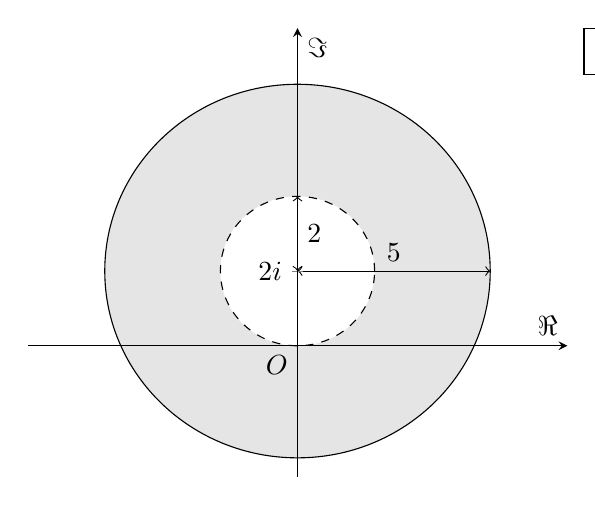
\begin{tikzpicture}[trim axis left, trim axis right]
                    \pgfdeclarelayer{pre main}
                    \pgfsetlayers{pre main,main}
                    \begin{axis}[
                        axis on top,
                        domain = 0:3 ,
                        samples = 101,
                        axis y line=middle,
                        axis x line=middle,
                        xtick = \empty,
                        ytick = {2},
                        yticklabels = {$2i$},
                        ymax=8.5,
                        ymin=-3.5,
                        xmin=-7,
                        xmax=7,
                        xlabel = {$\Re$},
                        ylabel = {$\Im$},
                        legend cell align={left},
                        legend pos=outer north east,
                        after end axis/.code={
                            \path (axis cs:0,0) 
                                node [anchor=north east] {$O$};
                            }
                        ]
                        \coordinate (Z1) at (0, 2);
                        \pgfonlayer{pre main}
                        \fill[black!10] (Z1) circle[radius=5];
                        \endpgfonlayer
                        \fill[white] (Z1) circle[radius=2];

                        \coordinate (O) at (0, 0);

                        \draw (Z1) circle[radius=5];
                        \draw[dashed] (Z1) circle[radius=2];

                        \addlegendimage{line legend, black!10, line width=5pt}
                        \addlegendentry{required locus};

                        \draw[<->] (Z1) -- (5, 2);
                        \draw[<->] (Z1) -- (0, 4);

                        \node[anchor=south] at (2.5, 2) {$5$};
                        \node[anchor=west] at (0, 3) {$2$};
                    \end{axis}
                \end{tikzpicture}
            \end{center}

        \part
            Note $\abs{z + i} > \abs{z + 1 - i} \implies \abs{z - (-i)} > \abs{z - (-1 + i)}$.

            \begin{center}
                \begin{tikzpicture}[trim axis left, trim axis right]
                    \pgfdeclarelayer{pre main}
                    \pgfsetlayers{pre main,main}
                    \begin{axis}[
                        axis on top,
                        domain = -4:10 ,
                        samples = 101,
                        axis y line=middle,
                        axis x line=middle,
                        xtick = \empty,
                        ytick = {-1},
                        yticklabels = {$-i$},
                        ymax=4,
                        ymin=-2,
                        xmin=-4.5,
                        xmax=2.5,
                        xlabel = {$\Re$},
                        ylabel = {$\Im$},
                        legend cell align={left},
                        legend pos=outer north east,
                        after end axis/.code={
                            \path (axis cs:0,0) 
                                node [anchor=north west] {$O$};
                            }
                        ]
                        \pgfonlayer{pre main}
                        \fill[black!10] (-4, -1.75) rectangle (2.5, 4);
                        \endpgfonlayer
                    
                        \coordinate[label=above left:$-1+i$] (Z1) at (-1, 1);
                        \coordinate (Z2) at (0, -1);

                        \addlegendimage{line legend, black!10, line width=5pt}
                        \addlegendentry{required locus};

                        \fill (Z1) circle[radius=2.5pt];
                        \fill (Z2) circle[radius=2.5pt];

                        \draw[dotted] (Z1) -- (Z2);
                        \addplot[dashed, black, name path=f1] {0.5 * x + 0.25};

                        \addplot[thin, name path=null, white] {-1.75};
                        \addplot[color=white] fill between[of=null and f1,soft clip={domain=-4:5}];

                        \coordinate (Z3) at (-0.5, 0);
                        \coordinate (Z4) at (0, 0.25);

                        \draw pic [draw, angle radius=3mm, ""] {right angle = Z4--Z3--Z1};
                    \end{axis}
                \end{tikzpicture}
            \end{center}

        \part
            Note $\dfrac\pi4 < \arg{\dfrac1z} \leq \dfrac\pi2 \implies \dfrac\pi4 < -\arg{z} \leq \dfrac\pi2 \implies -\dfrac\pi2 \geq \arg{z} > -\dfrac\pi4$.

            \begin{center}
                \begin{tikzpicture}[trim axis left, trim axis right]
                    \pgfdeclarelayer{pre main}
                    \pgfsetlayers{pre main,main}
                    \begin{axis}[
                        axis on top,
                        domain = -4:10 ,
                        samples = 101,
                        axis y line=middle,
                        axis x line=middle,
                        xtick = \empty,
                        ytick = \empty,
                        ymax=1,
                        ymin=-5,
                        xmin=-1,
                        xmax=7,
                        xlabel = {$\Re$},
                        ylabel = {$\Im$},
                        legend cell align={left},
                        legend pos=outer north east,
                        after end axis/.code={
                            \path (axis cs:0,0) 
                                node [anchor=north east] {$O$};
                            }
                        ]
                        \pgfonlayer{pre main}
                        \fill[black!10] (0, 0) rectangle (5, -5);
                        \endpgfonlayer

                        \addlegendimage{line legend, black!10, line width=5pt}
                        \addlegendentry{required locus};

                        \coordinate (O) at (0, 0);
                        \coordinate (Z1) at (5, -5);
                        \draw (O) circle[radius=2.5pt];

                        \addplot[dashed, domain=0:5, name path=f1] {-x};
                        
                        \addplot[thin, name path=null, white] {0};
                        \addplot[color=white] fill between[of=null and f1,soft clip={domain=0:5}];

                        \coordinate (Z2) at (5, 0);
                        \draw pic [draw, angle radius=12mm, "$-\frac\pi4$"] {angle = Z1--O--Z2};
                    \end{axis}
                \end{tikzpicture}
            \end{center}

    \problem{}
        Sketch on separate Argand diagrams for (a) and (b) the set of points representing all complex numbers $z$ satisfying both of the following inequalities.

        \begin{enumerate}
            \item $\abs{z - 3 - i} \leq 3$ and $\abs{z} \geq \abs{z - 3 - i}$
            \item $\dfrac\pi2 < \arg{z + 1} \leq \dfrac23 \pi$ and $3 \Im{z} > 2$
        \end{enumerate}

    \solution
        \part
            Note $\abs{z - 3 - i} \leq 3 \implies \abs{z - (3 + i)} \leq 3$ and $\abs{z} \geq \abs{z - 3 - i} \implies \abs{z} \geq \abs{z - (3 + i)}$.

            \begin{center}
                \begin{tikzpicture}[trim axis left, trim axis right]
                    \pgfdeclarelayer{pre main}
                    \pgfsetlayers{pre main,main}
                    \begin{axis}[
                        axis on top,
                        domain = -4:10 ,
                        samples = 101,
                        axis y line=middle,
                        axis x line=middle,
                        xtick = \empty,
                        ytick = \empty,
                        ymax=5,
                        ymin=-3,
                        xmin=-2,
                        xmax=7.5,
                        xlabel = {$\Re$},
                        ylabel = {$\Im$},
                        legend cell align={left},
                        legend pos=outer north east,
                        after end axis/.code={
                            \path (axis cs:0,0) 
                                node [anchor=north east] {$O$};
                            }
                        ]
                        \addlegendimage{line legend, black!10, line width=5pt}
                        \addlegendentry{required locus};

                        \coordinate (O) at (0, 0);
                        \coordinate[label=above:$3 + i$] (Z) at (3, 1);

                        \fill (O) circle[radius=2.5pt];
                        \fill (Z) circle[radius=2.5pt];
                        \draw (Z) circle[radius=3];

                        \draw[dotted] (O) -- (Z);

                        \pgfonlayer{pre main}
                            \fill[black!10] (Z) circle[radius=3];
                        \endpgfonlayer

                        
                        \addplot[black, name path=f1] {5 - 3*x};
                        \addplot[thin, name path=null, white] {-2.5};
                        \addplot[color=white] fill between[of=null and f1,soft clip={domain=0:6}];

                        \coordinate (Z1) at (0, 5);
                        \coordinate (Z2) at (1.5, 0.5);

                        \draw pic [draw, angle radius=3mm, ""] {right angle = Z1--Z2--O};

                        \draw[<->] (Z) -- (3, -2);
                        \node[anchor=west] at (3, -1) {$3$};
                    \end{axis}
                \end{tikzpicture}
            \end{center}

        \part
            Note $\dfrac\pi2 < \arg{z + 1} < \dfrac23 \pi \implies \dfrac\pi2 < \arg{z - (-1)} < \dfrac23 \pi$ and $3\Im{z} > 2 \implies \Im{z} > \dfrac23$.

            \begin{center}
                \begin{tikzpicture}[trim axis left, trim axis right]
                    \pgfdeclarelayer{pre main}
                    \pgfsetlayers{pre main,main}
                    \begin{axis}[
                        axis on top,
                        domain = -4:10 ,
                        samples = 101,
                        axis y line=middle,
                        axis x line=middle,
                        xtick = {-1},
                        ytick = {2/3},
                        yticklabels = {$\frac23 i$},
                        ymax=3,
                        ymin=-1,
                        xmin=-3,
                        xmax=1,
                        xlabel = {$\Re$},
                        ylabel = {$\Im$},
                        legend cell align={left},
                        legend pos=outer north east,
                        after end axis/.code={
                            \path (axis cs:0,0) 
                                node [anchor=north east] {$O$};
                            }
                        ]
                        \addlegendimage{line legend, black!10, line width=5pt}
                        \addlegendentry{required locus};

                        \coordinate (O) at (0, 0);
                        \coordinate (Z) at (-1, 0);

                        \fill (Z) circle[radius=2.5pt];

                        \pgfonlayer{pre main}
                            \fill[black!10] (-2, 2/3-0.01) rectangle (-1, 3);
                        \endpgfonlayer
                        
                        \addplot[black, name path=f1, domain=-3:-1, dashed] {-3*(x + 1)};
                        \addplot[thin, name path=null, white] {2/3};
                        \addplot[color=white] fill between[of=null and f1,soft clip={domain=-3:-1}];

                        \addplot[dashed] {2/3};

                        \draw[dashed] (Z) -- (-1, 5);
                    \end{axis}
                \end{tikzpicture}
            \end{center}

    \problem{}
        Illustrate, in separate Argand diagrams, the set of points $z$ for which
        
        \begin{enumerate}
            \item $\Re{z^2} < 0$
            \item $\Im{z^3} > 0$
        \end{enumerate}

    \solution
        \part
            Let $z = r(\cos \t + i\sin\t)$, $0 \leq \t < 2\pi$. Then $\Re(z^2) < 0 \implies r^2\cos 2\t < 0 \implies \cos 2\t < 0 \implies 2\t \in \bp{\dfrac12\pi, \dfrac32\pi} \cup \bp{\dfrac52 \pi, \dfrac72 \pi} \implies \t \in \bp{\dfrac14\pi, \dfrac34 \pi} \cup \bp{\dfrac54 \pi, \dfrac74 \pi}$.

            \begin{center}
                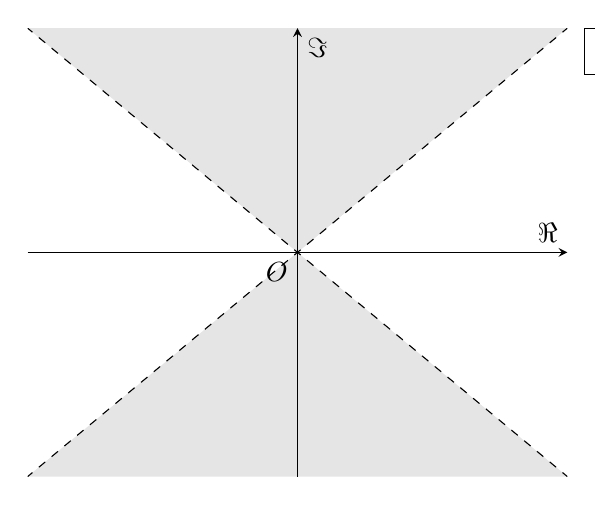
\begin{tikzpicture}[trim axis left, trim axis right]
                    \pgfdeclarelayer{pre main}
                    \pgfsetlayers{pre main,main}
                    \begin{axis}[
                        axis on top,
                        domain = -10:10 ,
                        samples = 101,
                        axis y line=middle,
                        axis x line=middle,
                        xtick = \empty,
                        ytick = \empty,
                        xmax=5,
                        xmin=-5,
                        ymin=-5,
                        ymax=5,
                        xlabel = {$\Re$},
                        ylabel = {$\Im$},
                        legend cell align={left},
                        legend pos=outer north east,
                        after end axis/.code={
                            \path (axis cs:0,0) 
                                node [anchor=north east] {$O$};
                            }
                        ]
                        \addlegendimage{line legend, black!10, line width=5pt}
                        \addlegendentry{required locus};
                        
                        \addplot[dashed] {x};
                        \addplot[dashed] {-x};

                        \pgfonlayer{pre main}
                            \fill[black!10] (-5, 5) -- (0, 0) -- (5, 5) -- cycle;
                            \fill[black!10] (-5, -5) -- (0, 0) -- (5, -5) -- cycle;
                        \endpgfonlayer
                    \end{axis}
                \end{tikzpicture}
            \end{center}

        \part
            Let $z = r(\cos \t + i\sin\t)$, $0 \leq \t < 2\pi$. Then $\Im(z^3) > 0 \implies r^3\sin 3\t > 0 \implies \sin 3\t > 0 \implies 3\t \in \bp{0, \pi} \cup \bp{2\pi, 3\pi} \cup \bp{4\pi, 5\pi} \implies \t \in \bp{0, \dfrac13 \pi} \cup \bp{\dfrac23 \pi, \pi} \cup \bp{\dfrac43\pi, \dfrac53 \pi}$.

            \begin{center}
                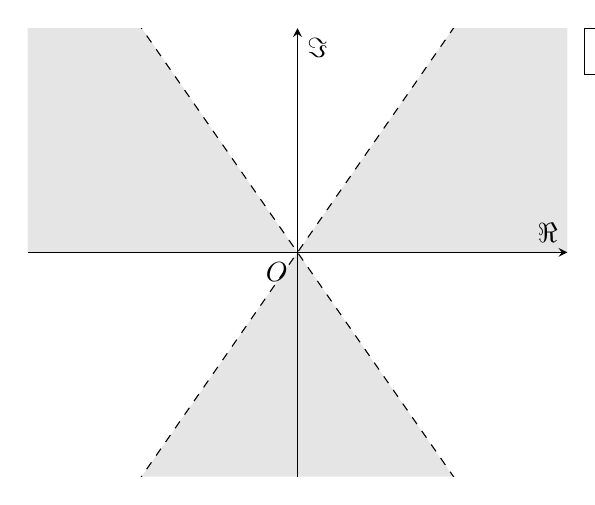
\begin{tikzpicture}[trim axis left, trim axis right]
                    \pgfdeclarelayer{pre main}
                    \pgfsetlayers{pre main,main}
                    \begin{axis}[
                        axis on top,
                        domain = -10:10 ,
                        samples = 101,
                        axis y line=middle,
                        axis x line=middle,
                        xtick = \empty,
                        ytick = \empty,
                        xmax=5,
                        xmin=-5,
                        ymin=-5,
                        ymax=5,
                        xlabel = {$\Re$},
                        ylabel = {$\Im$},
                        legend cell align={left},
                        legend pos=outer north east,
                        after end axis/.code={
                            \path (axis cs:0,0) 
                                node [anchor=north east] {$O$};
                            }
                        ]
                        \addlegendimage{line legend, black!10, line width=5pt}
                        \addlegendentry{required locus};
                        
                        \addplot[dashed] {1.73 * x};
                        \addplot[dashed] {-1.73 * x};

                        \pgfonlayer{pre main}
                            \fill[black!10] (5, 0) -- (0, 0) -- (2.886, 5) -- (5, 5) -- cycle;
                            \fill[black!10] (-5, 0) -- (0, 0) -- (-2.886, 5) -- (-5, 5) -- cycle;
                            \fill[black!10] (-2.886, -5) -- (0, 0) -- (2.886, -5) -- cycle;
                        \endpgfonlayer
                    \end{axis}
                \end{tikzpicture}
            \end{center}

    \problem{}
        The complex number $z$ satisfies $\abs{z + 4 - 4i} = 3$.
        \begin{enumerate}
            \item Describe, with the aid of a sketch, the locus of the point which represents $z$ in an Argand diagram.
            \item Find the least possible value of $\abs{z - i}$.
            \item Find the range of values of $\arg{z - i}$.
        \end{enumerate}
    
    \solution
        \part
            Note $\abs{z + 4 - 4i} = 3 \implies \abs{z - (-4 + 4i)} = 3$.

            \begin{center}
                \begin{tikzpicture}[trim axis left, trim axis right]
                    \begin{axis}[
                        domain = 0:10,
                        samples = 101,
                        axis y line=middle,
                        axis x line=middle,
                        xtick = \empty,
                        ytick = \empty,
                        xmax=1,
                        xmin=-8,
                        ymin=0,
                        ymax=8,
                        xlabel = {$\Re$},
                        ylabel = {$\Im$},
                        legend cell align={left},
                        legend pos=outer north east,
                        after end axis/.code={
                            \path (axis cs:0,0) 
                                node [anchor=north] {$O$};
                            }
                        ]
                        
                        \addlegendimage{no markers, plotRed}
                        \addlegendentry{required locus};

                        \coordinate[label=above:$C(-4 + 4i)$] (Z) at (-4, 4);
                        \coordinate (O) at (0, 0);
                        \coordinate[label=right:$I(i)$] (I) at (0, 1);
                              
                        \fill[name path=f1] (Z) circle[radius=2.5pt];
                        \fill (I) circle[radius=2.5pt];
                        
                        \draw[plotRed] (Z) circle[radius=3];

                        \draw[<->] (Z) -- (-4, 1);
                        \node[anchor=east] at (-4, 2.5) {$3$};

                        \draw[dotted] (I) -- (-8, 1);
                        \addplot[dotted, domain=-10:0, name path=f2] {-3.42335 * x + 1};

                        \coordinate[label=below:$A$] (A) at (-4, 1);
                        \coordinate[label=right:$B$] (B) at (-1.09, 4.746);

                        \fill (A) circle[radius=2.5pt];
                        \fill (B) circle[radius=2.5pt];
                        \draw[dotted] (I) -- (Z);

                        \draw pic [draw, angle radius=10mm, "$\t$"] {angle = Z--I--A};

                        \draw pic [draw, angle radius=12mm, "$\t$"] {angle = B--I--Z};
                    \end{axis}
                \end{tikzpicture}
            \end{center}

        \part
            Observe that the distance $CI$ is equal to the sum of the radius of the circle and $\min \abs{z - i}$. Hence,
            \[
                \min \abs{z - i} = \sqrt{(-4 - 0)^2 + (4 - 1)^2} - 3 = 2
            \]
            \boxt{$\min \abs{z - i} = 2$}

        \part
            Let $A$ and $B$ be points on the circle such that $AI$ and $BI$ are tangent to the circle. Let $\angle CIA = \t$. Then $\tan \t = \dfrac34 \implies \t = \arctan \dfrac34$. By symmetry, we also have $\angle CIB = \t$, whence $\angle AIB = 2\t = 2\arctan \dfrac34$. Hence, $\min \arg{z -i} = \pi - 2\arctan \dfrac34$ (at $B$) and $\max \arg{z - i} = \pi$ (at $A$).

            \boxt{$\pi - 2\arctan \dfrac34 \leq \arg{z-i} \leq \pi$}

    \problem{}
        Sketch, on the same Argand diagram, the two loci representing the complex number $z$ for which $z = 4 + ki$, where $k$ is a positive real variable, and $\abs{z - 1} = 4$. Write down, in the form $x + iy$, the complex number satisfying both conditions.

    \solution
        \begin{center}
            \begin{tikzpicture}[trim axis left, trim axis right]
                \begin{axis}[
                    domain = 0:10,
                    samples = 101,
                    axis y line=middle,
                    axis x line=middle,
                    xtick = {1, 4},
                    ytick = \empty,
                    xmax=6.75,
                    xmin=-4.75,
                    ymin=-5,
                    ymax=5,
                    xlabel = {$\Re$},
                    ylabel = {$\Im$},
                    legend cell align={left},
                    legend pos=outer north east,
                    after end axis/.code={
                        \path (axis cs:0,0) 
                            node [anchor=north east] {$O$};
                        }
                    ]
                    
                    \addlegendimage{no markers, plotBlue}
                    \addlegendentry{$\abs{z - 1} = 4$};

                    \addlegendimage{no markers, plotRed}
                    \addlegendentry{$z = 4 + ki$};

                    \draw[plotBlue] (1, 0) circle[radius=4];
                    \draw[plotRed] (4, 0) -- (4, 6);
                    \fill (1, 0) circle[radius=2.5pt];

                    \draw[<->] (1, 0) -- (1, 4);
                    \node[anchor=west] at (1, 2) {$4$};
                \end{axis}
            \end{tikzpicture}
        \end{center}

        Note that $z$ is of the form $4 + ki$, $k \in \R^+$. Since $\abs{z - 1} = 4$, we have $\abs{3 + ki} = 4 \implies 3^2 + k^2 = 4 \implies k = \sqrt7$. Note that we reject $k = -\sqrt7$ since $k > 0$.

        \boxt{$z = 4 + \sqrt7 i$}

    \problem{}
        Describe, in geometrical terms, the loci given by $\abs{z - 1} = \abs{z + i}$ and $\abs{z - 3 + 3i} = 2$ and sketch both loci on the same diagram.

        Obtain, in the form $a + ib$, the complex numbers representing the points of intersection of the loci, giving the exact values of $a$ and $b$.

    \solution
        Note that $\abs{z - 1} = \abs{z + i} \implies \abs{z - 1} = \abs{z - (-i)}$ and $\abs{z - 3 + 3i} = 2 \implies \abs{z - (3 - 3i)} = 2$.

        \boxt{\begin{center}The locus given by $\abs{z - 1} = \abs{z + i}$ is the perpendicular bisector of the line segment joining 1 and $-i$.\\The locus given by $\abs{z - 3 + 3i} = 2$ is a circle with centre $3 - 3i$ and radius 2.\end{center}}

        \begin{center}
            \begin{tikzpicture}[trim axis left, trim axis right]
                \begin{axis}[
                    domain = 0:10,
                    samples = 101,
                    axis y line=middle,
                    axis x line=middle,
                    xtick = {1},
                    ytick = {-1},
                    yticklabels = {$-i$},
                    xmax=7,
                    xmin=-1,
                    ymin=-6,
                    ymax=1,
                    xlabel = {$\Re$},
                    ylabel = {$\Im$},
                    legend cell align={left},
                    legend pos=outer north east,
                    after end axis/.code={
                        \path (axis cs:0,0) 
                            node [anchor=north east] {$O$};
                        }
                    ]
                    
                    \addlegendimage{no markers, plotRed}
                    \addlegendentry{$\abs{z - 1} = \abs{z + i}$};

                    \addlegendimage{no markers, plotBlue}
                    \addlegendentry{$\abs{z - 3 + 3i} = 2$};

                    \coordinate (Z1) at (1, 0);
                    \coordinate (Z2) at (0, -1);
                    \coordinate[label=left:$3-3i$] (C) at (3, -3);

                    \fill (C) circle[radius=2.5pt];

                    \draw[dotted] (Z1) -- (Z2);
                    \draw[plotRed] (-1, 1) -- (6, -6);

                    \draw[plotBlue] (C) circle[radius=2];                    
                \end{axis}
            \end{tikzpicture}
        \end{center}

        Observe that the locus of $\abs{z - 1} = \abs{z + i}$ has Cartesian equation $y = -x$ and the locus of $\abs{z - 3 + 3i} = 2$ has Cartesian equation $(x-3)^2 + (y+3)^2 = 2^2$. Solving both equations simultaneously, we have
        \begin{alignat*}{2}
            &&(x-3)^2 + (y+3)^2 &= 2^2\\
            \implies&&(x-3)^2 + (3-x)^2 &= 4\\
            \implies&&x^2 - 6x + 9 + 9 - 6x + x^2 &= 4\\
            \implies&&2x^2 - 12x + 14 &= 0\\
            \implies&&x^2 - 6x + 7 &= 0\\
            \implies&&x &= \dfrac{6 \pm \sqrt{8}}{2}\\
            && &= 3 \pm \sqrt2\\
            \implies&&y &= -(3 \pm \sqrt2)\\
            && &= -3 \mp \sqrt2
        \end{alignat*}
        Hence, the complex numbers representing the points of intersections of the loci are $(3 + \sqrt2) + (-3 - \sqrt2)i$ and $(3 - \sqrt2) + (-3 + \sqrt2)i$.

        \boxt{$(3 + \sqrt2) + (-3 - \sqrt2)i$, $(3 - \sqrt2) + (-3 + \sqrt2)i$}

    \problem{}
        Sketch the locus for $\arg{z - (4\sqrt3 - 2i)} = \dfrac56\pi$ in an Argand diagram.

        \begin{enumerate}
            \item Verify that the points $2i$ and $2\sqrt3$ lie on it.
            \item Find the minimum value of $\abs{z}$ and the range of values of $\arg{z}$.
        \end{enumerate}

    \solution
        \begin{center}
            \begin{tikzpicture}[trim axis left, trim axis right]
                \begin{axis}[
                    domain = 0:10,
                    samples = 101,
                    axis y line=middle,
                    axis x line=middle,
                    xtick = \empty,
                    ytick = {2},
                    yticklabels = {$A(2i)$},
                    xmax=9,
                    xmin=-1,
                    ymin=-4,
                    ymax=4,
                    xlabel = {$\Re$},
                    ylabel = {$\Im$},
                    legend cell align={left},
                    legend pos=outer north east,
                    after end axis/.code={
                        \path (axis cs:0,0) 
                            node [anchor=north east] {$O$};
                        }
                    ]
                    
                    \addlegendimage{no markers, plotRed}
                    \addlegendentry{required locus};

                    \coordinate[label=above right:$B(2\sqrt3)$] (B) at (3.46, 0);
        
                    \coordinate[label=below:$4\sqrt3 - 2i$] (Z) at (6.928, -2);
                    \coordinate (O) at (0, 0);
                        
                    \draw (Z) circle[radius=2.5pt];

                    \addplot[plotRed, domain=-1:6.928] {-0.577 * x + 2};

                    \coordinate (Z1) at (12, -2);
                    \coordinate (Z2) at (0, 2);

                    \fill (Z2) circle[radius=2.5pt];
                    \fill (3.464, 0) circle[radius=2.5pt];

                    \draw[dotted] (Z1) -- (Z);
                    \draw pic [draw, angle radius=7mm, "$\frac56 \pi$"] {angle = Z1--Z--Z2};

                    \addplot[domain=0:0.85, dotted] {1.73 * x};

                    \coordinate[label=above right:$C$] (C) at (0.87, 1.48);
                    \fill (C) circle[radius=2.5pt];

                    \draw pic [draw, angle radius=3mm, ""] {right angle = B--C--O};

                    \draw[dotted] (O) -- (Z);
                \end{axis}
            \end{tikzpicture}
        \end{center}
        
        \part
            \[
                \arg{2i - (4\sqrt3 - 2i)} = \arg{-\sqrt3 + i} = \arctan \dfrac1{-\sqrt3} = \dfrac56\pi
            \]
            \[
                \arg{2\sqrt3 - (4\sqrt3 - 2i)} = \arg{-\sqrt3 + i} = \arctan \dfrac1{-\sqrt3} = \dfrac56\pi
            \]
            Hence, the points $2i$ and $2\sqrt3$ satisfy the equation $\arg{z - (4\sqrt3 - 2i)} = \dfrac56\pi$ and thus lie on the locus.

        \part
            Let $A(2i)$ and $B(2\sqrt3)$. Let $C$ be the point on the required locus such that $OC \perp AB$. Observe that $\triangle OAB$, $\triangle COB$ and $\triangle CAO$ are all similar to one another. Hence,
            \[
                \dfrac{OC}{CB} = \dfrac{AO}{BO} = \dfrac1{\sqrt3} \implies AC = \dfrac1{\sqrt3} OC
            \]
            \[
                \dfrac{OC}{CA} = \dfrac{BO}{OA} = \dfrac{\sqrt3}1 \implies BC = \sqrt3 OC
            \]
            Hence, $AB = AC + CB = \bp{\sqrt3 + \dfrac1{\sqrt3}} OC \implies \min \abs{z} = OC = \dfrac{AB}{\sqrt3 + 1/\sqrt3} = \dfrac{\sqrt{2^2 + (2\sqrt3)^2}}{\sqrt3 + 1\sqrt{3}} = \dfrac{4\sqrt3}{4} = \sqrt3$.
            \boxt{$\min \abs{z} = \sqrt3$}
            
            Observe that $\max \arg{z} = \dfrac56 \pi$ and $\min \arg{z} = \min \arg{4\sqrt3 - 2i} = \arctan \dfrac{-2}{4\sqrt3} = -\arctan \dfrac1{2\sqrt3}$.
            \boxt{$-\arctan \dfrac1{2\sqrt3} < \arg{z} \leq \dfrac56 \pi$}


    \problem{}
        The complex number $z$ satisfies $\abs{z - 3 - 3i} \geq \abs{z - 1 - i}$ and $\dfrac\pi6 < \arg{z} \leq \dfrac\pi3$.

        \begin{enumerate}
            \item On an Argand diagram, sketch the region in which the point representing $z$ can lie.
            \item Find the area of the region in part (a).
            \item Find the range of values of $\arg{z - 5 + i}$.
        \end{enumerate}
    
    \solution
        \part
            Note that $\abs{z - 3 - 3i} \leq \abs{z - 1 - i} \implies \abs{z - (3 + 3i)} \leq \abs{z - (1 + i)}$.

            \begin{center}
                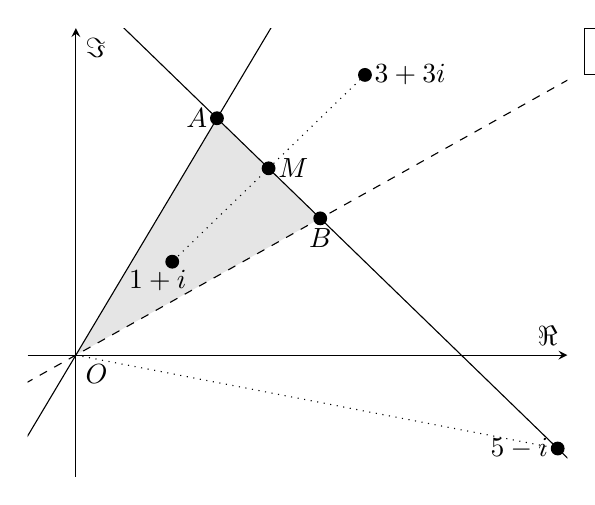
\begin{tikzpicture}[trim axis left, trim axis right]
                    \pgfdeclarelayer{pre main}
                    \pgfsetlayers{pre main,main}
                    \begin{axis}[
                        axis on top,
                        domain = -10:10 ,
                        samples = 101,
                        axis y line=middle,
                        axis x line=middle,
                        xtick = \empty,
                        ytick = \empty,
                        xmax=6/1.25 + 0.3,
                        xmin=-1/1.25 + 0.3,
                        ymin=-2/1.25 + 0.3,
                        ymax=4/1.25 + 0.3,
                        xlabel = {$\Re$},
                        ylabel = {$\Im$},
                        legend cell align={left},
                        legend pos=outer north east,
                        after end axis/.code={
                            \path (axis cs:0,0) 
                                node [anchor=north west] {$O$};
                            }
                        ]
                        \addlegendimage{line legend, black!10, line width=5pt}
                        \addlegendentry{required locus};
                        
                        \addplot[black] {-x + 4};
                        \addplot[black] {1.73 * x};
                        \addplot[dashed] {0.577 * x};

                        \coordinate (O) at (0, 0);
                        \coordinate[label=left:$A$] (A) at (1.464, 2.536);
                        \coordinate[label=below:$B$] (B) at (2.536, 1.464);

                        \pgfonlayer{pre main}
                            \fill[black!10] (0, 0) -- (A) -- (B) -- cycle;
                        \endpgfonlayer

                        \coordinate[label=right:$3 + 3i$] (Z1) at (3, 3);
                        \coordinate (Z2) at (1, 1);
                        \draw[dotted] (Z1) -- (Z2);

                        \node at (0.85, 0.8) {$1 + i$};

                        \fill (A) circle[radius=2.5pt];
                        \fill (B) circle[radius=2.5pt];
                        \fill (Z1) circle[radius=2.5pt];
                        \fill (Z2) circle[radius=2.5pt];

                        \coordinate[label=left:$5 - i$] (Z3) at (5, -1);
                        \fill (Z3) circle[radius=2.5pt];
                        
                        \draw[dotted] (O) -- (Z3);

                        \coordinate[label=right:$M$] (M) at (2, 2);
                        \fill (M) circle[radius=2.5pt];
                    \end{axis}
                \end{tikzpicture}
            \end{center}

        \part
            Note that the locus of $\abs{z - 3 - 3i} = \abs{z - 1 - i}$ has Cartesian equation $y = -x + 4$, while the loci of $\dfrac\pi6 = \arg{z}$ and $\arg{z} = \dfrac\pi3$ have Cartesian equations $y = \dfrac1{\sqrt3} x$ and $y = \sqrt3 x$ respectively. Let $A$ and $B$ be the intersections between $y = -x + 4$ with $y = \sqrt3 x$ and $y = \dfrac1{\sqrt3}x$ respectively.

            At $A$, we have $y = \sqrt3 x = -x + 4$, whence $A\bp{\dfrac4{1 + \sqrt3}, \dfrac{4\sqrt3}{1 + \sqrt3}}$. At $B$, we have $y = \dfrac1{\sqrt3}x = -x + 4$, whence $B\bp{\dfrac{4\sqrt3}{1 + \sqrt3}, \dfrac4{1 + \sqrt3}}$. Observe that $M\bp{2, 2}$ is the midpoint of $AB$. Then the required area is given by $\dfrac12 \cdot AB \cdot OM$.
            {\allowdisplaybreaks
            \begin{align*}
                \area &= \dfrac12 \cdot AB \cdot OM\\
                &= \dfrac12 \cdot \sqrt{\bp{\dfrac4{1 + \sqrt3} - \dfrac{4\sqrt3}{1 + \sqrt3}}^2 + \bp{\dfrac{4\sqrt3}{1 + \sqrt3} - \dfrac4{1 + \sqrt3}}^2} \cdot \sqrt{2^2 + 2^2}\\
                &= \dfrac12 \cdot \sqrt{2\bp{\dfrac4{1 + \sqrt3} - \dfrac{4\sqrt3}{1 + \sqrt3}}^2} \cdot 2\sqrt2\\
                &= 2 \cdot \abs{\dfrac4{1 + \sqrt3} - \dfrac{4\sqrt3}{1 + \sqrt3}}\\
                &= 8 \cdot \abs{\dfrac{1 - \sqrt3}{1 + \sqrt3}}\\
                &= 8 \cdot \abs{\dfrac{(1 - \sqrt3)^2}{(1 + \sqrt3)(1 - \sqrt3)}}\\
                &= 8 \cdot \abs{\dfrac{(1 - \sqrt3)^2}{-2}}\\
                &= 4 (1 - \sqrt3)^2
            \end{align*}}

            \boxt{The area of the region is $4(1 - \sqrt3)^2$ units$^2$.}

        \part
            Note that $\arg{z - 5 + i} = \arg{z - (5 - i)}$. Observe that $\min \arg{z - (5 - i)} = \dfrac34 \pi$ and $\max \arg{z - (5 -i)} = \arctan \dfrac{-1}5 + \pi = \pi -\arctan \dfrac15 $.

            \boxt{$\dfrac34 \pi \leq \arg{z - 5 + i} < \pi-\arctan \dfrac15$}

    \problem{}
        Sketch on an Argand diagram the set of points representing all complex numbers $z$ satisfying both inequalities
        \[
            \abs{iz - 2i - 2} \leq 2 \qquad \text{and} \qquad \Re{z} > \abs{1 + \sqrt3 i}
        \]
        Find
        \begin{enumerate}
            \item the range of $\arg{z - 2 - 2i}$,
            \item the complex number $z$ where $\arg{z - 2 - 2i}$ is a maximum.
        \end{enumerate}

        The locus of the complex number $w$ is defined by $\abs{w - 5 + 2i} = k$, where $k$ is a real and positive constant. Find the range of values of $k$ such that the loci of $w$ and $z$ will intersect.

    \solution
        Note $\abs{iz - 2i - 2} \leq 2 \implies \abs{i (z - 2 + 2i)} \leq 2 \implies \abs{z - (2 - 2i)} \leq 2$ and $\Re{z} > \abs{1 + \sqrt3 i} = 2$. 
        
        \begin{center}
            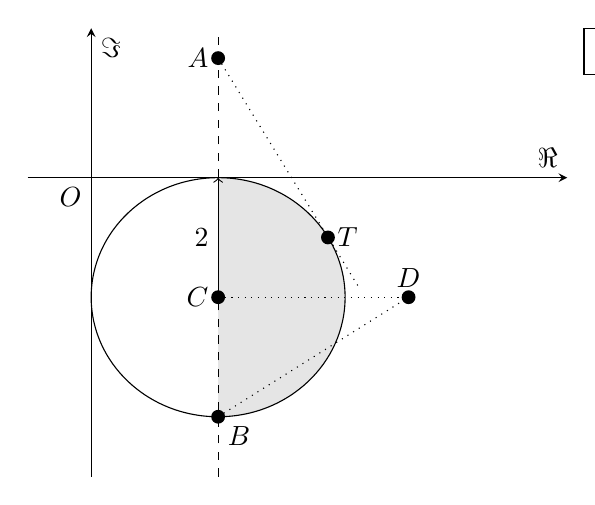
\begin{tikzpicture}[trim axis left, trim axis right]
                \pgfdeclarelayer{pre main}
                \pgfsetlayers{pre main,main}
                \begin{axis}[
                    axis on top,
                    domain = -10:10 ,
                    samples = 101,
                    axis y line=middle,
                    axis x line=middle,
                    xtick = \empty,
                    ytick = \empty,
                    xmax=7.5,
                    xmin=-1,
                    ymin=-5,
                    ymax=2.5,
                    xlabel = {$\Re$},
                    ylabel = {$\Im$},
                    legend cell align={left},
                    legend pos=outer north east,
                    after end axis/.code={
                        \path (axis cs:0,0) 
                            node [anchor=north east] {$O$};
                        }
                    ]
                    \addlegendimage{line legend, black!10, line width=5pt}
                    \addlegendentry{required locus};

                    \coordinate[label=left:$C$] (C) at (2, -2);
                    \draw (C) circle[radius=2];
                    \coordinate[label=above:$D$] (Z) at (5, -2);

                    \fill (C) circle[radius=2.5pt];
                    \fill (Z) circle[radius=2.5pt];

                    \draw[dashed] (2, -5) -- (2, 2.5);

                    \pgfonlayer{pre main}
                        \fill[black!10] (C) circle[radius=2];
                        \fill[white] (2, -4.5) rectangle (0, 0);
                    \endpgfonlayer

                    \draw[<->] (C) -- (2, 0);
                    \node[anchor=east] at (2, -1) {2};

                    \coordinate[label=below right:$B$] (B) at (2, -4);
                    \draw[dotted] (C) -- (Z);
                    \draw[dotted] (B) -- (Z);
                    \fill (B) circle[radius=2.5pt];

                    \coordinate[label=left:$A$] (A) at (2, 2);
                    \fill (A) circle[radius=2.5pt];

                    \addplot[dotted, domain=2:4.2] {-1.73 * (x-2) + 2};

                    \fill (2 + 1.73, -1) circle[radius=2.5pt] node[anchor=west] {$T$};
                \end{axis}
            \end{tikzpicture}
        \end{center}

        \part
            Note $\abs{z - 2 - 2i} = \arg{z - (2 + 2i)}$. Let $A(2 + 2i)$ and $C(2 - 2i)$. Let $T$ be the point at which $AT$ is tangent to the circle. Then $\angle ATC = \dfrac\pi2$, $AC = 4$ and $TC = 2$. Hence, $\angle CAT = \arcsin \dfrac24 = \dfrac\pi6$. Thus, $\min \arg{z - 2 - 2i} = -\dfrac\pi2$ and $\max \arg{z - 2 - 2i} = \min \arg{z - 2 - 2i} + \angle CAT = -\dfrac\pi2 + \dfrac\pi6 = -\dfrac\pi3$.

            \boxt{$-\dfrac\pi2 < \arg{z - 2 - 2i} \leq -\dfrac\pi3$}
                      
        \part
            Relative to $C$, $T$ is given by $2 \bp{\cos \dfrac\pi6 + i\sin \dfrac\pi6} = \sqrt3 + i$. Thus, $T = (\sqrt 3 + i) + (2 - 2i) = 2 + \sqrt3 - i$.

            \boxt{$2 + \sqrt3 - i$}

        
        Note $\abs{w - 5 + 2i} = k \implies \abs{w - (5 - 2i)} = k$. Let $D(5 - 2i)$. Observe that $CD$ is given by the sum of the radius of the circle and $\min k$. Hence, $\min k = 3 - 2 = 1$. Let $B(2 - 4i)$. Then $\max k$ is given by the distance between $B$ and $D$. By the Pythagorean Theorem, we have $\max k = \sqrt{(5-2)^2 + (-2-(-4))^2} = \sqrt{13}$.

        \boxt{$1 \leq k \leq \sqrt{13}$}
\end{document}